\subsection{Robustness to assumptions about rapid test sensitivity}
\label{subsec:robustness_rapid_test_sensitivity}


Our result that frequent and large scale rapid testing was responsible for a
large decrease in cases in the spring of 2021 in Germany seems to be at odds
with the general perception that rapid tests are unreliable. They also seem to
contradict recent studies showing that the actual sensitivity of rapid tests t
be lower than advertised (e.g.\cite{Scheiblauer2021}).

This is, however, not the case. It is important to distinguish studies that
analyze the sensitivity and specificity of rapid tests in isolation and studies
that analyze the aggregate effect of testing strategies within an
epidemiological model.

This section shows that our results are robust to making less favorable
assumptions on rapid test sensitivity. We proceed by describing several possible
ways of calibrating rapid test sensitivity profiles based on recent studies.
Since none of these methods is inherently better than the others, we make
simulations with two sensitivity profiles: The average over all methods and the
lower envelope over all methods.

Both profiles imply much lower sensitivities of rapid tests than used in our
main results, especially in the later stage of an infection. However, the main
results stay very robust. The original result was that rapid tests, seasonality
and vaccinations are responsible for 42\%, 43\% and 16\%, respectively. With the
average profile, the effect of rapid tests goes down to 41 \%. With the lower
envelope profile, which is an extremely unfavorable assumption, it becomes 38\%.


% what do we need
The effect of rapid tests on infection dynamics strongly depends on \emph{when}
an infection is detected. Earlier detection means that it is more likely that
the infection has not yet been discovered for a different reason (e.g. due to
the onset of symptoms) and that the infected person can be isolated before
spreading the disease to others.

The sensitivity of rapid tests depends on the viral load in the repiratory
tract. It is low at the beginning of an infection (especially before the onset
of infectiousness), high in the first few days of infectiousness and then
gradually decreasing towards the end of infectiousness.

We thus need to calibrate a profile of rapid test sensitivities based on the
number of days until or since the onset of infectiousness.

% what is available -> two step mapping
Unfortunately, such sensitivity profiles are not usually reported in studies. We
thus need to create them by combining two types of studies: 1. Studies that
report the viral load in terms of threshold cycle ($C_t$) values determined by
PCR test (e.g. \cite{Cosentino2022}, \cite{Ong2021}, \cite{Bonnet2022},
\cite{Jang2021} and \cite{Zuin2021}). 2. Studies that report the ensitivity of
rapid tests for different $C_t$ values (e.g. \cite{Scheiblauer2021},
\cite{Bruemmer2021}).


% what options do we have to configure the mappings
It is natural to assume that the evolution of $C_t$ values over time as well as
the effect of $C_t$ values on rapid test sensitivity are continuous functions.
However, the results of the available studies are usually reported in a
discretized way. This leads to multiple ways of calculating the sensitivity
profiles. Some try to recover the underlying continuous functions using
interpolation or regression, others simply use the discretized values.

% Describe CT value formula vs. bin averages
For the calibration of $C_t$ values over time we can either use discretized
values for several time bins from \cite{Ong2021} and \cite{Jang2021}.
Alternatively, we can use linearized formulas for calculating sensitivities over
time \cite{Cosentino2022}.

% Describe sensitivity lookupd vs. interpolation
For the mapping of $C_t$ values to rapid test sensitivities, again we have two
options. First, we can simply look up the discretized values for the three $C_t$
provided in \cite{Scheiblauer2021} (below 20, 25 to 30 and above 35). Secondly,
we can use linear regression to estimate a continous mapping for the
relationship by assuming that the $C_t$ values of each bin are achieved exactly
at the bin midpoints and that the relationship is linear.

% Properties of the different methods
In general, using discretized values can lead to an underestimation of peak
sensitivities and an overestimation of very low sensitivities. This is because
discretization is essentially a smoothing device. On the other hand, it hat the
advantage of simply working with published results, without introducing any
tuning parameters or other assumptions.


% resulting profiles.
\begin{figure}
    \centering
    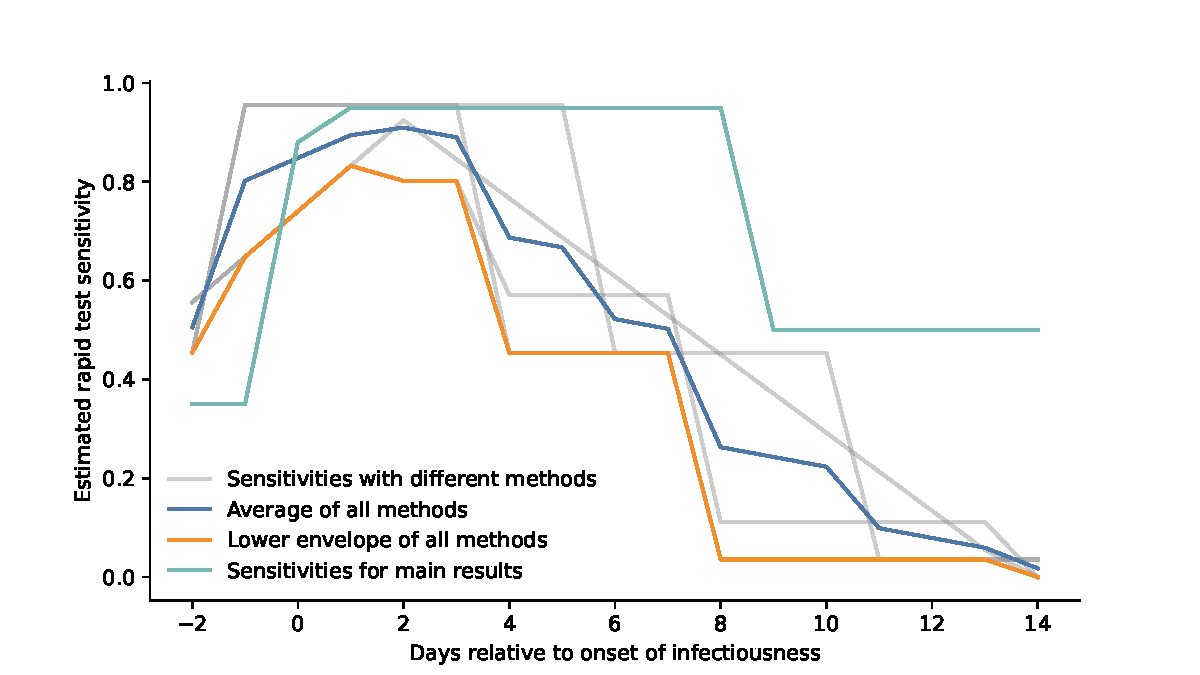
\includegraphics[width=0.9\textwidth]{figures/results/figures/data/testing/sensitivity_params_with_different_methods}
    \caption{Rapid test sensitivity profiles}
    \floatfoot{\noindent \textit{Note:} The figure shows estimated sensitivities
    of rapid tests over the course of an infection. The x-axis shows days
    relative to the onset of infectiousness. The y-axis shows the estimated
    rapid test sensitivities. The grey lines are the raw sensitivity estimates
    obtained with different methods of dealing with discretized data. The blue
    line shows their average and the yellow line their lower envelope. The
    turquoise line are the sensitivities used for the main results of the paper.
    It is much higher than the new estimates in the later stage of an infection.
    Luckily this has only a very small effect on the overall effectiveness of
    rapid tests on the infection dynamics.}
    \label{fig:sensitivity_assumptions}
\end{figure}

\FloatBarrier


Figure \ref{fig:sensitivity_assumptions} shows that the updated sensitivity
estimates are lower than the ones used for our original results, especially
towards the end of an infection. However, the main results barely change.




\begin{figure}
    \centering

    \begin{subfigure}[b]{0.475\textwidth}
        \centering
        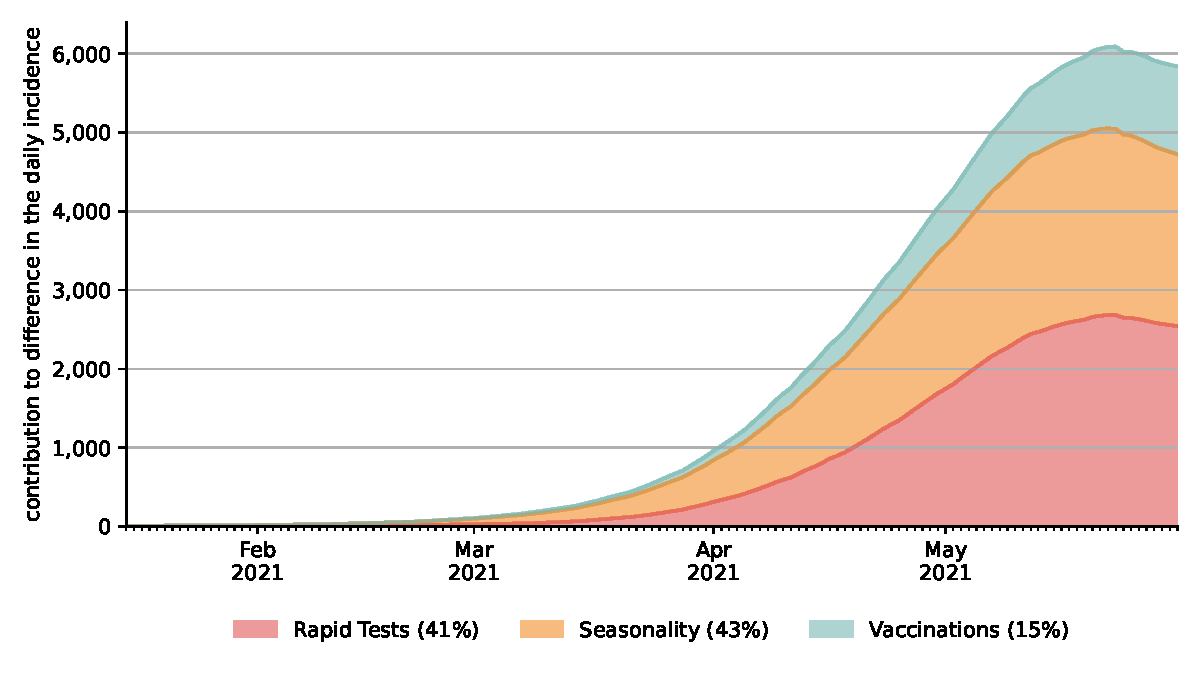
\includegraphics[width=0.9\textwidth]{figures/results/figures/data/testing/full_decomposition_channels_area_average}
        \caption{Shapley decomposition with average of sensitivity estimates}
    \end{subfigure}
    \begin{subfigure}[b]{0.475\textwidth}
        \centering
        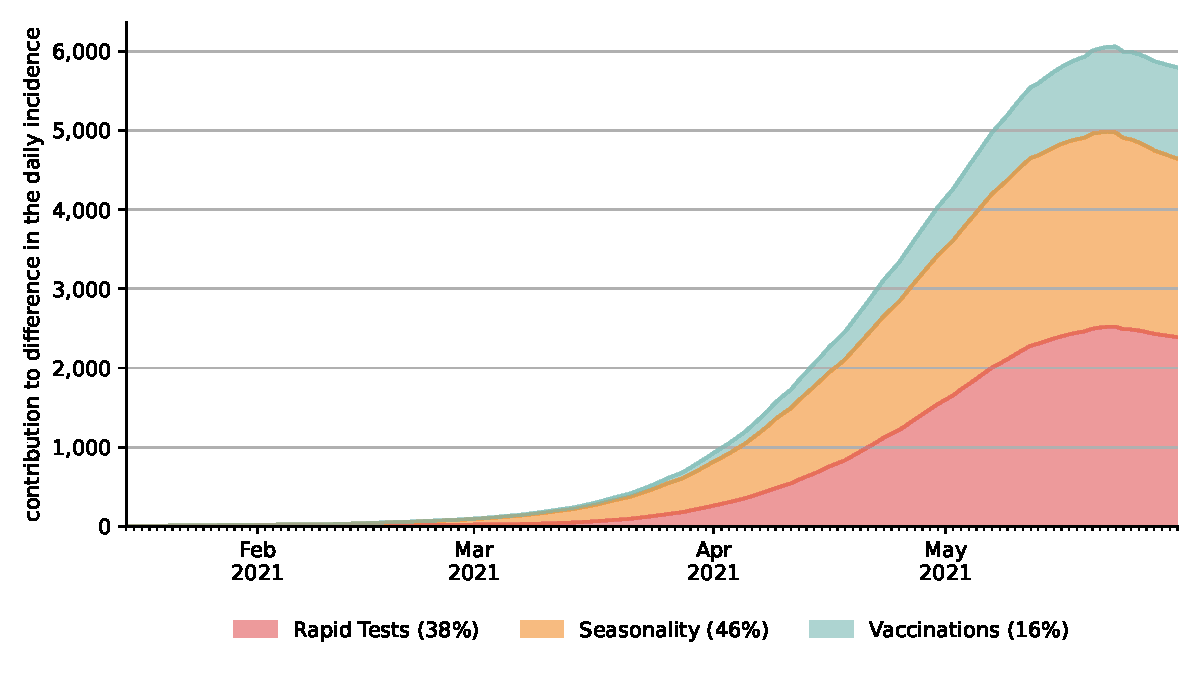
\includegraphics[width=0.9\textwidth]{figures/results/figures/data/testing/full_decomposition_channels_area_lower_envelope}
        \caption{Shapley decomposition with lower envelope of sensitivity estimates}
    \end{subfigure}

    \caption{Updated shapley decompositions}
    \floatfoot{\noindent \textit{Note:} The figure shows updated versions of the
    shapley decomposition in figure \ref{fig:2021_scenarios_decomposition}. The
    decomposition is based on 20 model runs with different random seeds. The
    share attributed to each channel is rounded to the next full percentage
    point to acknowledge the remaining sampling uncertainty.}
    \label{fig:robustness_to_sensitivity_assumptions}
\end{figure}

\FloatBarrier

%


